% UCL Thesis LaTeX Template
%  (c) Ian Kirker, 2014
% 
% This is a template/skeleton for PhD/MPhil/MRes theses.
%
% It uses a rather split-up file structure because this tends to
%  work well for large, complex documents.
% We suggest using one file per chapter, but you may wish to use more
%  or fewer separate files than that.
% We've also separated out various bits of configuration into their
%  own files, to keep everything neat.
% Note that the \input command just streams in whatever file you give
%  it, while the \include command adds a page break, and does some
%  extra organisation to make compilation faster. Note that you can't
%  use \include inside an \include-d file.
% We suggest using \input for settings and configuration files that
%  you always want to use, and \include for each section of content.
% If you do that, it also means you can use the \includeonly statement
%  to only compile up the section you're currently interested in.
% You might also want to put figures into their own files to be \input.

% For more information on \input and \include, see:
%  http://tex.stackexchange.com/questions/246/when-should-i-use-input-vs-include


% Formatting rules for theses are here: 
%  http://www.ucl.ac.uk/current-students/research_degrees/thesis_formatting
% Binding and submitting guidelines are here:
%  http://www.ucl.ac.uk/current-students/research_degrees/thesis_binding_submission

% This package goes first and foremost, because it checks all 
%  your syntax for mistakes and some old-fashioned LaTeX commands.
% Note that normally you should load your documentclass before 
%  packages, because some packages change behaviour based on
%  your document settings.
% Also, for those confused by the RequirePackage here vs usepackage
%  elsewhere, usepackage cannot be used before the documentclass
%  command, while RequirePackage can. That's the only functional
%  difference as far as I'm aware.
\RequirePackage[l2tabu, orthodox]{nag}

% ------ Main document class specification ------
% The draft option here prevents images being inserted,
%  and adds chunky black bars to boxes that are exceeding 
%  the page width (to show that they are).
% The oneside option can optionally be replaced by twoside if
%  you intend to print double-sided. Note that this is
%  *specifically permitted* by the UCL thesis formatting
%  guidelines.
%
% Valid options in terms of type are:
%  phd
%  mres
%  mphil
%\documentclass[12pt,phd,draft,a4paper,oneside]{ucl_thesis}
\documentclass[12pt,mphil,a4paper,oneside]{ucl_thesis}

% Package configuration:
%  LaTeX uses "packages" to add extra commands and features.
%  There are quite a few useful ones, so we've put them in a 
%   separate file.
% -------- Packages --------

% This package just gives you a quick way to dump in some sample text.
% You can remove it -- it's just here for the examples.
\usepackage{blindtext}

% This package means empty pages (pages with no text) won't get stuff
%  like chapter names at the top of the page. It's mostly cosmetic.
\usepackage{emptypage}

% The graphicx package adds the \includegraphics command,
%  which is your basic command for adding a picture.
\usepackage{graphicx}

% The float package improves LaTeX's handling of floats,
%  and also adds the option to *force* LaTeX to put the float
%  HERE, with the [H] option to the float environment.
\usepackage{float}

% The amsmath package enhances the various ways of including
%  maths, including adding the align environment for aligned
%  equations.
\usepackage{amsmath}

% Use these two packages together -- they define symbols
%  for e.g. units that you can use in both text and math mode.
\usepackage{gensymb}
\usepackage{textcomp}
% You may also want the units package for making little
%  fractions for unit specifications.
%\usepackage{units}


% The setspace package lets you use 1.5-sized or double line spacing.
\usepackage{setspace}
\setstretch{1.5}

% That just does body text -- if you want to expand *everything*,
%  including footnotes and tables, use this instead:
%\renewcommand{\baselinestretch}{1.5}


% PGFPlots is either a really clunky or really good way to add graphs
%  into your document, depending on your point of view.
% There's waaaaay too much information on using this to cover here,
%  so, you might want to start here:
%   http://pgfplots.sourceforge.net/
%  or here:
%   http://pgfplots.sourceforge.net/pgfplots.pdf
%\usepackage{pgfplots}
%\pgfplotsset{compat=1.3} % <- this fixed axis labels in the version I was using

% PGFPlotsTable can help you make tables a little more easily than
%  usual in LaTeX.
% If you're going to have to paste data in a lot, I'd suggest using it.
%  You might want to start with the manual, here:
%  http://pgfplots.sourceforge.net/pgfplotstable.pdf
%\usepackage{pgfplotstable}

% These settings are also recommended for using with pgfplotstable.
%\pgfplotstableset{
%	% these columns/<colname>/.style={<options>} things define a style
%	% which applies to <colname> only.
%	empty cells with={--}, % replace empty cells with '--'
%	every head row/.style={before row=\toprule,after row=\midrule},
%	every last row/.style={after row=\bottomrule}
%}


% The mhchem package provides chemistry formula typesetting commands
%  e.g. \ce{H2O}
%\usepackage[version=3]{mhchem}

% And the chemfig package gives a weird command for adding Lewis 
%  diagrams, for e.g. organic molecules
%\usepackage{chemfig}

% The linenumbers command from the lineno package adds line numbers
%  alongside your text that can be useful for discussing edits 
%  in drafts.
% Remove or comment out the command for proper versions.
%\usepackage[modulo]{lineno}
% \linenumbers 


% Alternatively, you can use the ifdraft package to let you add
%  commands that will only be used in draft versions
%\usepackage{ifdraft}

% For example, the following adds a watermark if the draft mode is on.
%\ifdraft{
%  \usepackage{draftwatermark}
%  \SetWatermarkText{\shortstack{\textsc{Draft Mode}\\ \strut \\ \strut \\ \strut}}
%  \SetWatermarkScale{0.5}
%  \SetWatermarkAngle{90}
%}


% The multirow package adds the option to make cells span 
%  rows in tables.
\usepackage{multirow}


% Subfig allows you to create figures within figures, to, for example,
%  make a single figure with 4 individually labeled and referenceable
%  sub-figures.
% It's quite fiddly to use, so check the documentation.
%\usepackage{subfig}

% The natbib package allows book-type citations commonly used in
%  longer works, and less commonly in science articles (IME).
% e.g. (Saucer et al., 1993) rather than [1]
% More details are here: http://merkel.zoneo.net/Latex/natbib.php
%\usepackage{natbib}

% The bibentry package (along with the \nobibliography* command)
%  allows putting full reference lines inline.
%  See: 
%   http://tex.stackexchange.com/questions/2905/how-can-i-list-references-from-bibtex-file-in-line-with-commentary
\usepackage{bibentry} 

% The isorot package allows you to put things sideways 
%  (or indeed, at any angle) on a page.
% This can be useful for wide graphs or other figures.
%\usepackage{isorot}

% The caption package adds more options for caption formatting.
% This set-up makes hanging labels, makes the caption text smaller
%  than the body text, and makes the label bold.
% Highly recommended.
\usepackage[format=hang,font=small,labelfont=bf]{caption}

% If you're getting into defining your own commands, you might want
%  to check out the etoolbox package -- it defines a few commands
%  that can make it easier to make commands robust.
\usepackage{etoolbox}

\usepackage{tabularx}

\usepackage{graphicx}
\usepackage{url}
\usepackage{color}
\usepackage[utf8]{inputenc}
\usepackage{amsmath}

\usepackage{tabularx} 
\setlength\extrarowheight{2pt} % make the tables look less cramped
\usepackage{graphicx}
\usepackage{adjustbox}
\newcommand{\ca}{\mbox{C$\alpha$}}
\newcommand{\VH}{\mbox{V\kern-.1667em \lower.5ex\hbox{\scriptsize H}}}
\newcommand{\VL}{\mbox{V\kern-.1667em \lower.5ex\hbox{\scriptsize L}}}
\newcommand{\VHVL}{\mbox{\VH/\VL}}
\newcommand{\CH}[1]{\mbox{C\lower.5ex\hbox{\scriptsize H}#1}}
\newcommand{\CL}{\mbox{C\kern-.0833em \lower.5ex\hbox{\scriptsize L}}}
\newcommand{\FV}{\mbox{\it Fv}}
\newcommand{\Fab}{\mbox{\it Fab}}

\newcommand{\e}[1]{\mbox{$\times 10^{#1}$}}
\newcommand{\etal}{~\emph{et al.}}
\newcommand{\degree}{\mbox{${}^{\circ}$}}
\newcommand{\lilian}[1]{ {\color{red}{\bfseries Lilian:} #1}}
\newcommand{\andrew}[1]{ {\color{green}{\bfseries Andrew:} #1}}
\newcommand{\rewrite}[1]{{\color{blue}{\bfseries Andrew to rewrite:} #1}}

\usepackage{soul}
\newcommand{\highlight}[1]{\hl{#1}}
% \newcommand{\highlight}[1]{{\color{cyan} #1}} % Use this if soul package not available!

\let\shortcite\cite
\emergencystretch 1in


% Sets up links within your document, for e.g. contents page entries
%  and references, and also PDF metadata.
% You should edit this!
%%
%% This file uses the hyperref package to make your thesis have metadata embedded in the PDF, 
%%  and also adds links to be able to click on references and contents page entries to go to 
%%  the pages.
%%

% Some hacks are necessary to make bibentry and hyperref play nicely.
% See: http://tex.stackexchange.com/questions/65348/clash-between-bibentry-and-hyperref-with-bibstyle-elsart-harv
\usepackage{bibentry}
\makeatletter\let\saved@bibitem\@bibitem\makeatother
\usepackage[pdftex,hidelinks]{hyperref}
\makeatletter\let\@bibitem\saved@bibitem\makeatother
\makeatletter
\AtBeginDocument{
    \hypersetup{
        pdfsubject={Thesis Subject},
        pdfkeywords={Thesis Keywords},
        pdfauthor={Author},
        pdftitle={Title},
    }
}
\makeatother
    


% And then some settings in separate files.
% These settings are from:
%  http://mintaka.sdsu.edu/GF/bibliog/latex/floats.html

% They give LaTeX more options on where to put your figures, and may
%  mean that fewer of your figures end up at the tops of pages far
%  away from the thing they're related to.

% Alters some LaTeX defaults for better treatment of figures:
% See p.105 of "TeX Unbound" for suggested values.
% See pp. 199-200 of Lamport's "LaTeX" book for details.

%   General parameters, for ALL pages:
\renewcommand{\topfraction}{0.9}	% max fraction of floats at top
\renewcommand{\bottomfraction}{0.8}	% max fraction of floats at bottom

%   Parameters for TEXT pages (not float pages):
\setcounter{topnumber}{2}
\setcounter{bottomnumber}{2}
\setcounter{totalnumber}{4}     % 2 may work better
\setcounter{dbltopnumber}{2}    % for 2-column pages
\renewcommand{\dbltopfraction}{0.9}	% fit big float above 2-col. text
\renewcommand{\textfraction}{0.07}	% allow minimal text w. figs

%   Parameters for FLOAT pages (not text pages):
\renewcommand{\floatpagefraction}{0.7}	% require fuller float pages
% N.B.: floatpagefraction MUST be less than topfraction !!
\renewcommand{\dblfloatpagefraction}{0.7}	% require fuller float pages

% remember to use [htp] or [htpb] for placement,
% e.g. 
%  \begin{figure}[htp]
%   ...
%  \end{figure} % For things like figures and tables
\bibliographystyle{unsrt}   % For bibliographies

% These control how many number sections your subsections will take
%    e.g. Section 2.3.1.5.6.3
%  and how many of those will get put into the contents pages.
\setcounter{secnumdepth}{3}
\setcounter{tocdepth}{3}


\begin{document}

\nobibliography*
% ^-- This is a dumb trick that works with the bibentry package to let
%  you put bibliography entries whereever you like.
% I used this to put references to papers a chapter's work was 
%  published in at the end of that chapter.
% For more information, see: http://stefaanlippens.net/bibentry

% If you haven't finished making your full BibTex file yet, you
%  might find this useful -- it'll just replace all your
%  citations with little superscript notes.
% Uncomment to use.
%\renewcommand{\cite}[1]{\emph{\textsuperscript{[#1]}}}

% At last, content! Remember filenames are case-sensitive and 
%  *must not* include spaces.
% I may change the way this is done in a future version, 
%  but given that some people needed it, if you need a different degree title 
%  (e.g. Master of Science, Master in Science, Master of Arts, etc)
%  uncomment the following 3 lines and set as appropriate (this *has* to be before \maketitle)
% \makeatletter
% \renewcommand {\@degree@string} {Master of Things}
% \makeatother

\title{Upgrade Report}
\author{Lilian Denzler}
\department{UCL Department of Structural and Molecular Biology}

\maketitle


\begin{Overview} % 300 word limit

The following report summarizes two projects: The T-Cell Receptor Numbering Project, as well as the Qualiloop project. 
In the first instance, a software package was created to reliably number T-Cell Receptor sequences. An accurate numbering package is essential for future proposed project within the PhD. The guiding idea for this section is to re-create a numbering system such as the in-house software used to number antibody sequences, applied to TCRs. 

Secondly, a 3D-model quality predictor of a Complementary Determining Rgion (CDR-H3) is presented. Machine learning techniques are implemented to predict the accuracy of CDR-H3 3D-models generated by antibody modelling software such as abYmod. The predictor is made available at \url{http://www.bioinf.org.uk/abs/qualiloop/}. 

Lastly, future directions for the PhD project are explored. 

\end{Overview}

%\begin{acknowledgements}
%I am hugely grateful to my primary supervisor Prof. Andrew Martin and chair of my committee for the invaluable patience %and feedback. I would also like to thank my secondary supervisor Prof. Adrian Shepherd and my tertiary supervisor Prof. %Benny Chain, who provided their expertise and guidance. Additionally, this endeavor would not have been possible without %the generous support from the MRC, who financed my research. Lastly, I would like to thank Immunocore, the iCASE %collaborating industrial partner. 

%\end{acknowledgements}

\setcounter{tocdepth}{2} 
% Setting this higher means you get contents entries for
%  more minor section headers.

\tableofcontents
%\listoffigures
%\listoftables


%\chapter{Introductory Material}
\label{chapterlabel1}
A robust sequence numbering method for T-cell receptors is important for all work with T-cell receptor sequence data. Universal numbering schemes and correct residue numbering is vital for sequence analysis and comparison. We present a numbering software for T-cell receptor sequences that will reliably implement a set of popular numbering schemes. The software also enables T-cell receptor sequences to be labeled using numbering schemes commonly used for antibodies, which will facilitate studying the differences and commonalities of T-cell receptors and antibodies. It will also enable antibody-based tools to be adapted to T-cell receptor sequences. The numbering software is made available at http://www.bioinf.org.uk/abs/

 

\chapter{T-Cell Receptor Sequence Numbering}
\label{chapterlabel1}
A robust sequence numbering method for T-cell receptors is important for all work with T-cell receptor sequence data. Universal numbering schemes and correct residue numbering is vital for sequence analysis and comparison. We present a numbering software for T-cell receptor sequences that will reliably implement a set of popular numbering schemes. The software also enables T-cell receptor sequences to be labeled using numbering schemes commonly used for antibodies, which will facilitate studying the differences and commonalities of T-cell receptors and antibodies. It will also enable antibody-based tools to be adapted to T-cell receptor sequences. The numbering software is to be made available at \url{http://www.bioinf.org.uk/abs/qualiloop/TCRnum}


Reliable sequence numbering is vital for sequence analysis and comparison. Given the lack of a universally agreed upon numbering scheme to be implemented for T-cell receptor sequences, sequence comparisons can be non-trivial. 
If TCR sequences can also be correctly numbered using schemes commonly implemented for antibody sequences, this will facilitate further research into the likeness of antibody and TCR-characteristics. 
In a paper comparing antibody and TCR CDRs,\cite{Wong2019} it was found that TCR and antibody CDRs occupy distinct areas of structural space. Understanding more about how the two relate may lead to a greater understanding of TCR and their functionality. 
The most commonly used antibody numbering schemes are arguably Kabat-, and Chothia-numbering. Therefore, numbering TCRs using these systems would be of great value for comparing TCR and antibody sequences. IMGT and Aho numbering, as two additional popular numbering schemes,will also be prove useful. 
Furthermore, having correctly numbered TCRs using the same numbering schemes commonly used for antibody sequences will facilitate the re-writing of antibody-geared tools created by Prof. Martin for TCRs. 
There are not many publicly available options available for TCR sequence numbering. An example of already existing software is ANARCI\cite{Dunbar2016}, which is a numbering tool that handles antibody as well as TCR sequences of human or murine origin. TCR sequences may be numbered according to Aho or IMGT schemes.  Furthermore, an unpublished numbering tool can be found on the tcrdb server\cite{Chen2021}, which offers a choice of Kabat or Aho numbering. However, the methods and accuracy of this tool are not publicly available. Therefore, the generation of reliable, robust numbering software that can utilize the Kabat, Chothia, IMGT and Aho scheme, would be very useful for future projects involving TCR sequences. This is especially true, when one considers the fact that all further sequence analyses is subject to correct numbering.

\section{Results}

Firstly, a web interface was created to interactively display different numbering schemes interactively. The different numbering schemes can be selected, as well as the chain type. Insertion/deletion sites according to the selected numbering scheme are denoted, as well as the CDR locations based on Kabat definitions transferred to the TCR context \ref{fig:schemes}. 
\begin{figure}
    \centering
    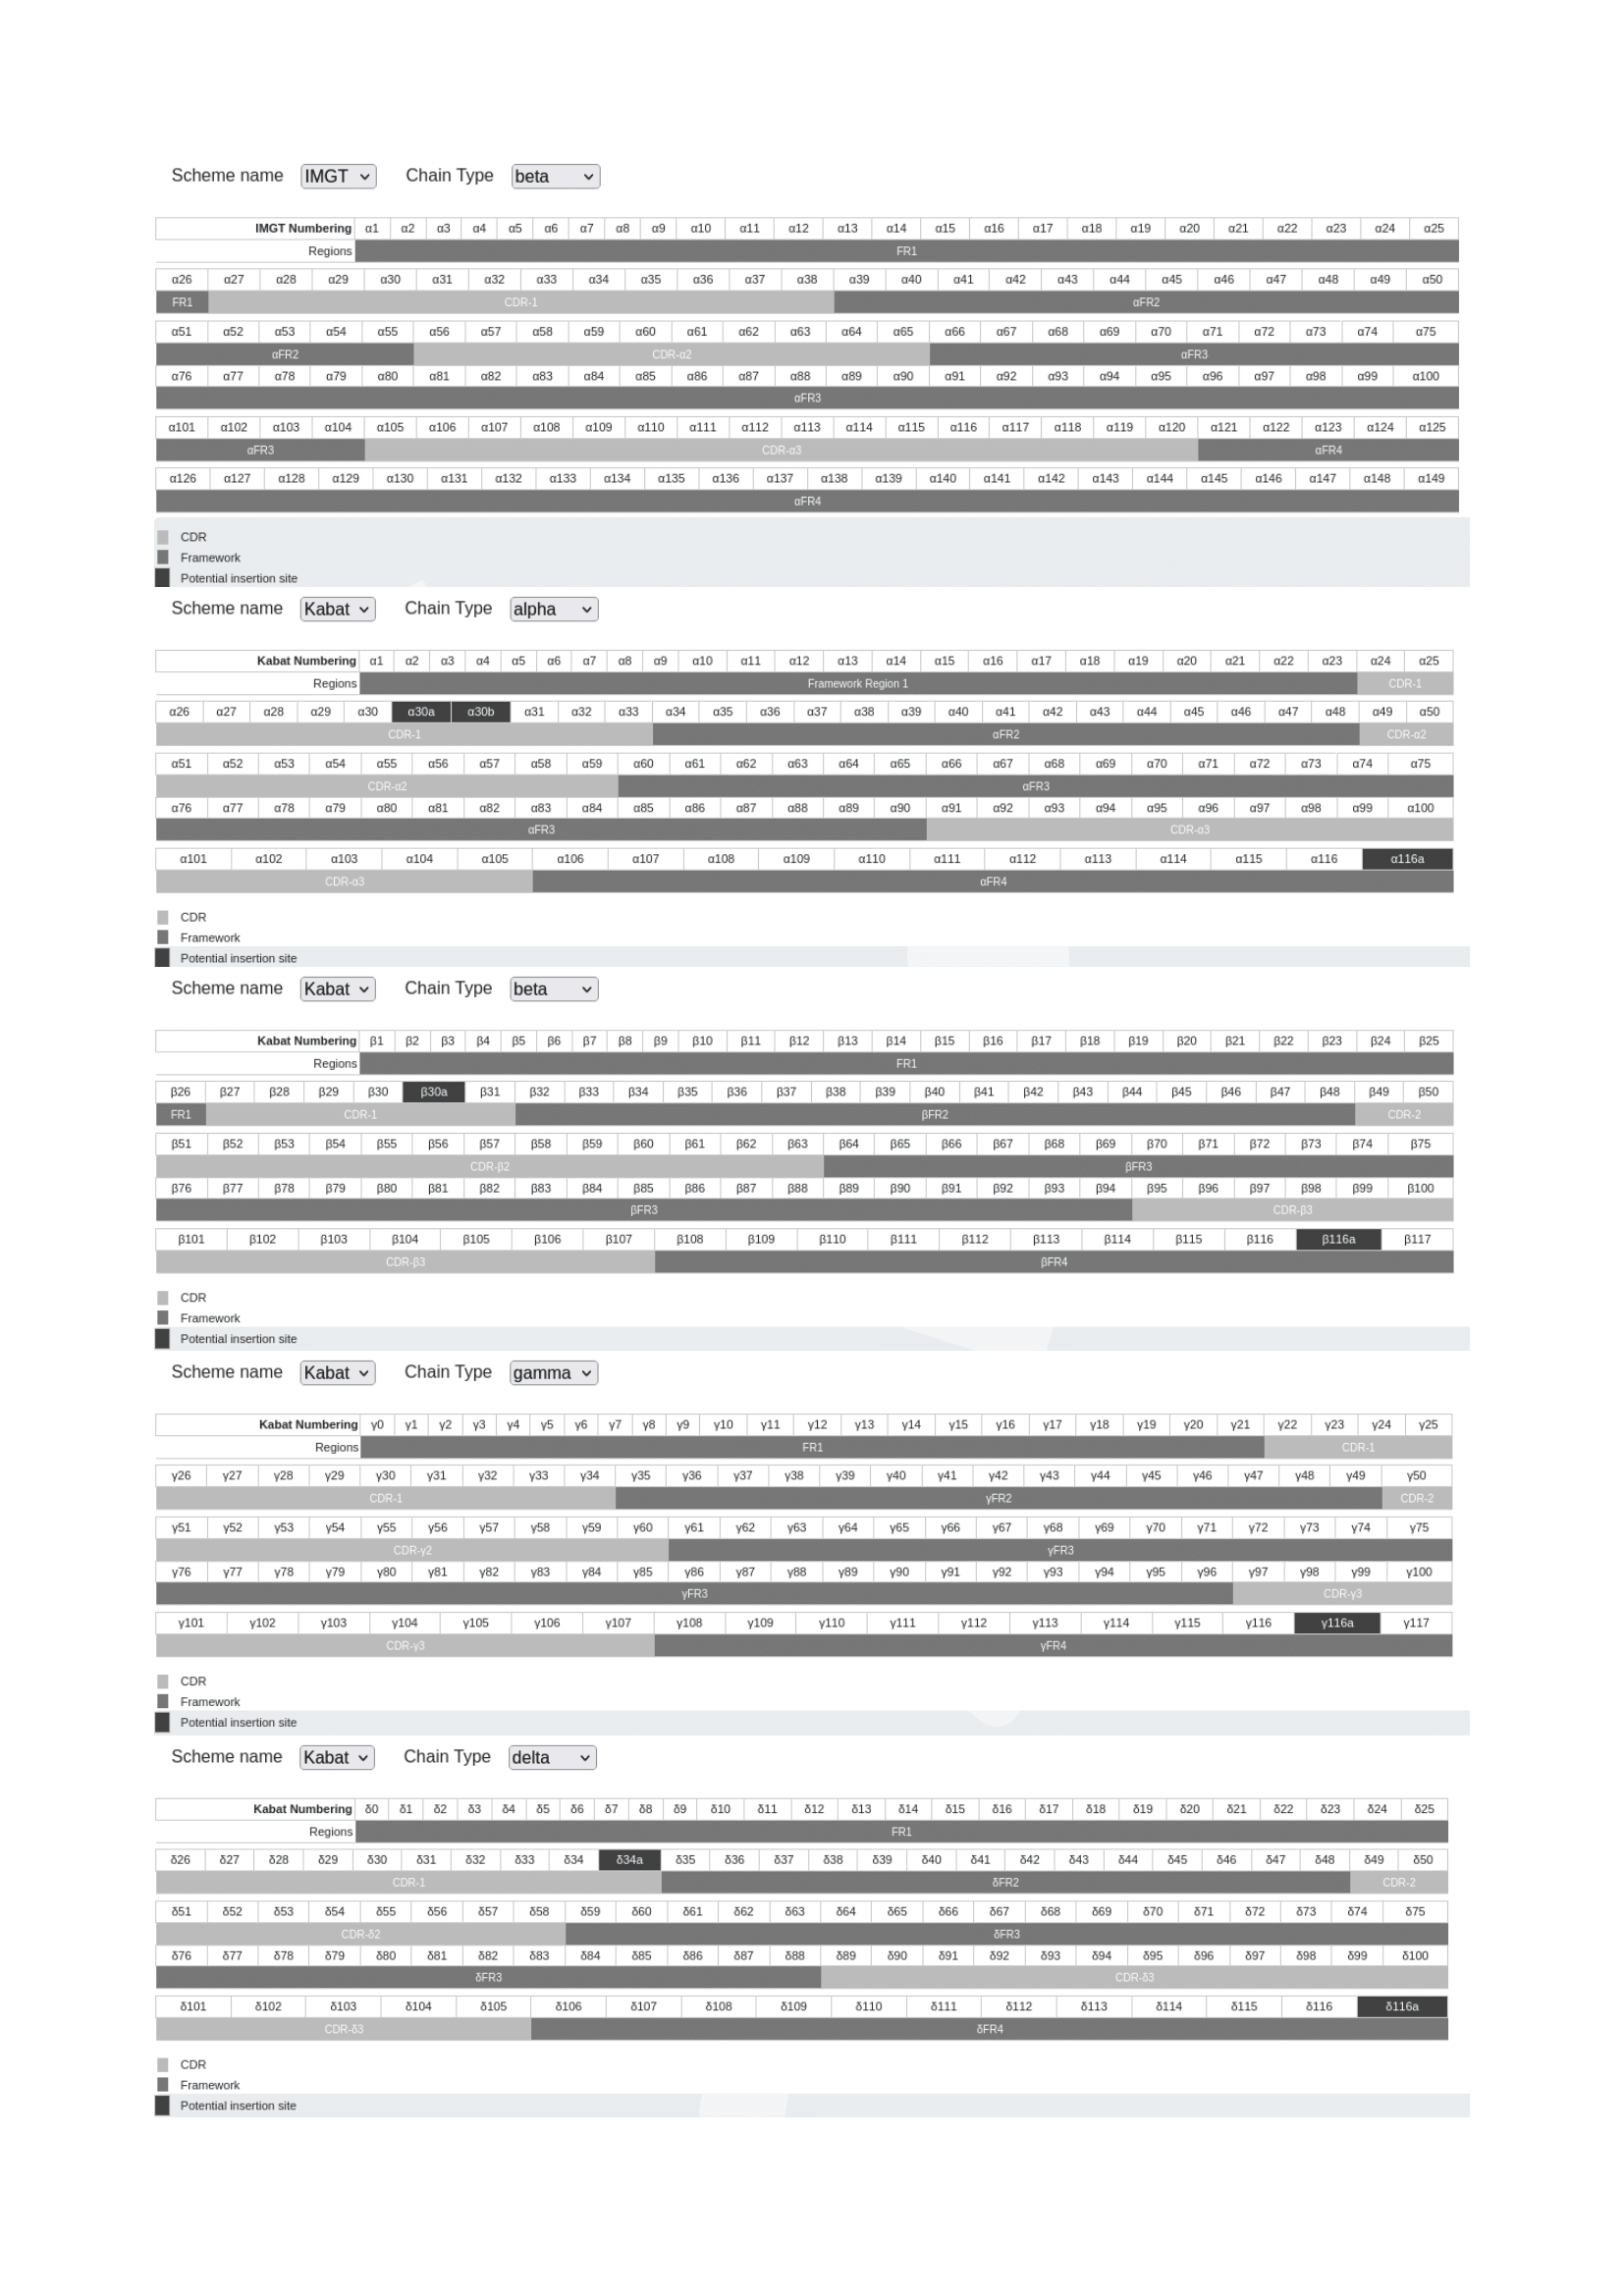
\includegraphics[width=\textwidth,height=\textheight,keepaspectratio]{schemes-1.png}
    \caption{The different numbering schemes for TCR sequences. The placement of insertions/deletions and position of the complementarity determining regions implied by the numbering scheme are displayed. (Not all numbering schemes are displayed here. For the complete set visit \url{http://www.bioinf.org.uk/abs/qualiloop/TCRnum} }
    \label{fig:schemes}
\end{figure}

In order to obtain a reliable numbering programme, a set of correctly numbered sequences for each of the numbering schemes is needed. These sequences are sorted by chain type and organism and are stored in MongoDB database collections along with the correct numbering \ref{fig:database_creation} Once the database is set up, the CDR regions within the different numbering schemes are defined. As no official Kabat or Chothia definitions of the CDR regions exist, these were arrived at using an alignment with the equivalent antibody numbering scheme\cite{AAAAA}.
Furthermore, by analysing the sequences in the newly produced mongo database, a Kabat-style definition for the TCR can be proposed \ref{fig:Aho_logo}, \ref{fig:IMGT_logo}.

\begin{figure}
    \centering
    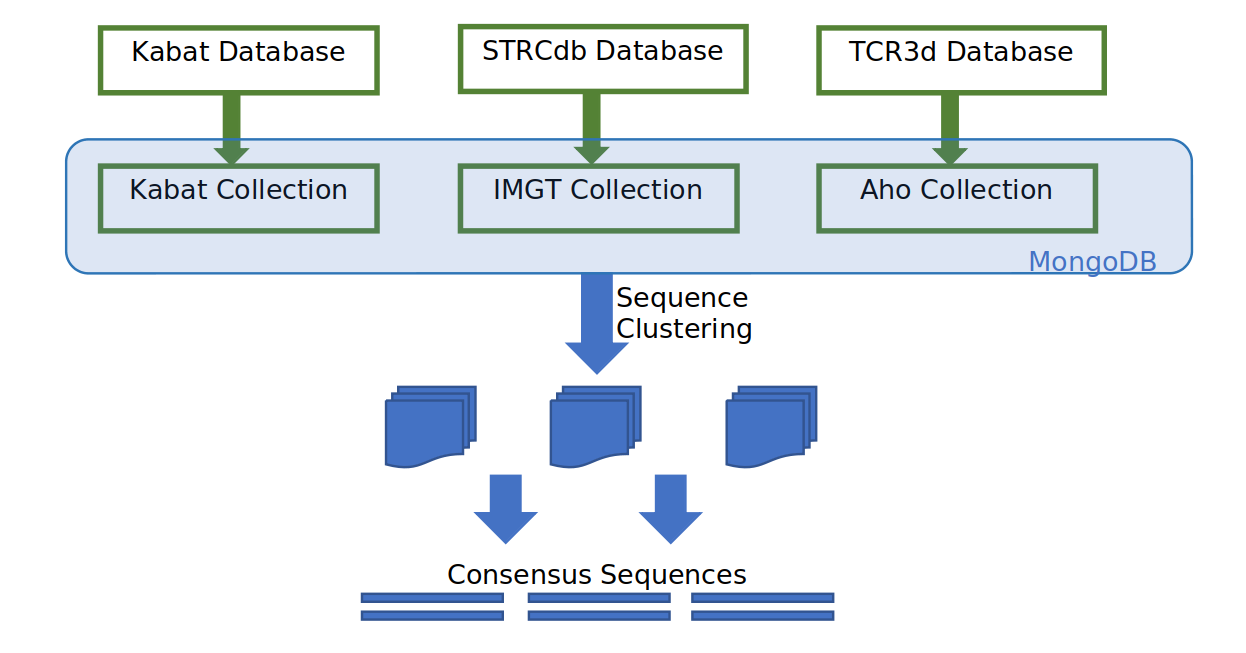
\includegraphics[width=\textwidth,height=\textheight,keepaspectratio]{database_creation.png}
    \caption{Consensus Sequence Creation. First, a MongoDB database is created, with three collections. These contain the parsed sequences with their meta data of Kabat, IMGT and Aho pre-numbered sequence databases. The sequences are then clustered (categorized by chain type). Residue frequency is analysed among the clusters to yield multiple consensus sequences, as well as conserved sequences.}
    \label{fig:database_creation}
\end{figure}


\begin{figure}
    \centering
    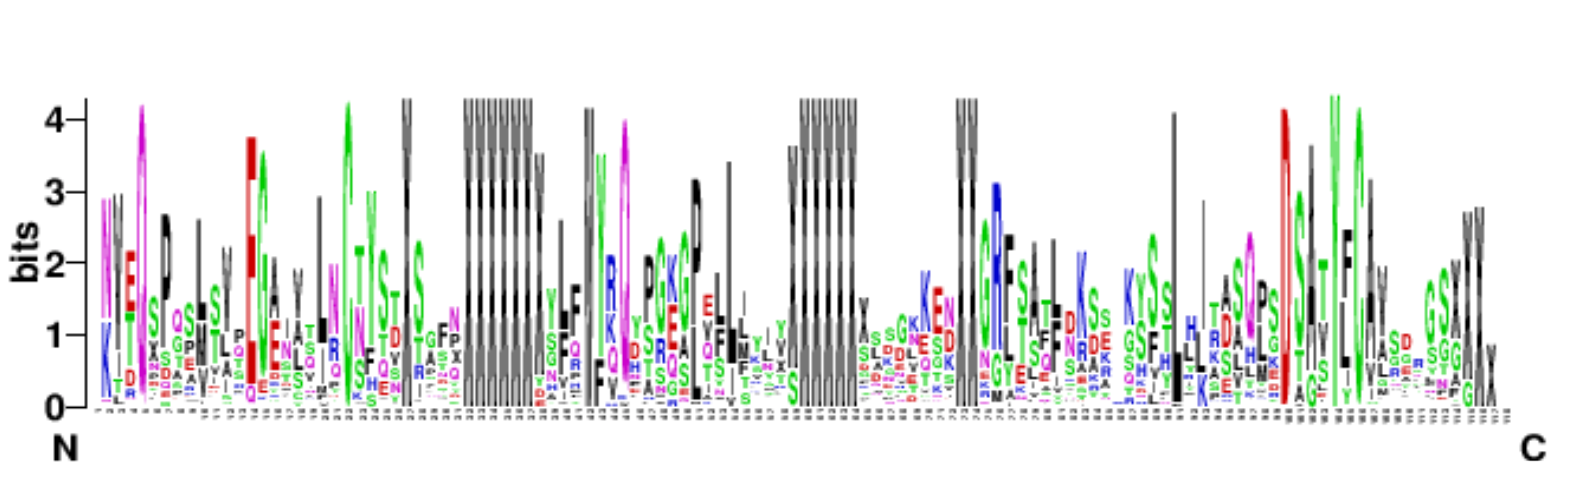
\includegraphics[width=\textwidth,height=\textheight,keepaspectratio]{Aho_logo.png}
    \caption{ Sequence Logo of TCR sequences in tcr3d database (Aho-numbered). Few conserved residues can be seen, as well as areas of greater sequence variability. Although some interesting features may be seen within this logo, there are many partial sequences in the  tcr3d database,which may distort some regions. }
    \label{fig:Aho_logo}
\end{figure}

\begin{figure}
    \centering
    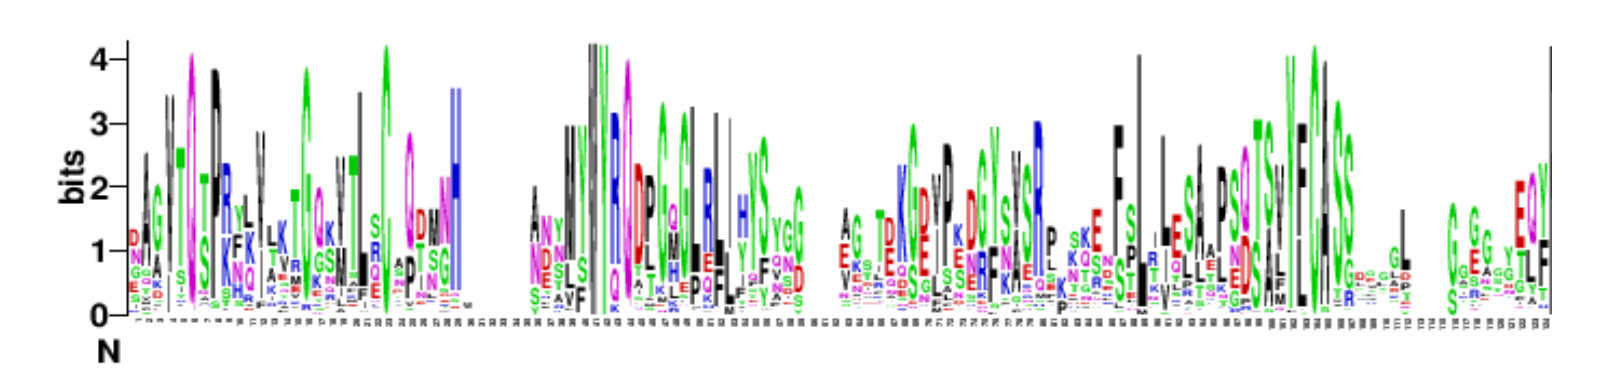
\includegraphics[width=\textwidth,height=\textheight,keepaspectratio]{IMGT_logo.png}
    \caption{Sequence Logo of TCR sequences in STRCdb database (IMGT-numbered). Few conserved residues can be seen, as well as areas of greater sequence variability. A similarity with Figure 2 can be seen. (Note:  the two figures have not been aligned according to sequence).}
    \label{fig:IMGT_logo}
\end{figure}

A consensus sequence can also be obtained for these sequences. Through prior sequence clustering by sequence identity, more informative consensus sequences can be produced\ref{fig:database_creation} The best-matching consensus sequence will then be selected for each sequence that is to be numbered in further steps. 

\subsection{Anchor Sequence Alignment}
In this equivalent to the AbNum-algorithm, sequence propensity profiles which are aligned to the sequence to find the CDR boundaries are used. By aligning short anchor sequences (10 \AA) built from sequence propensity profiles before and after CDR regions, the numbering can be filled in. The amino acid numbers are filled in from both sides in turn.

The sequence propensity profiles were built for each of the framework regions and CDRs using all organisms and chain types. Then, profiles were build for FR and CDRs separated by chain type, then separated by organism and lastly by both organism and chain type. 

[Most reliably, a large set of profiles separated by both organism and chain type will be used. The best match is selected for the first anchor alignment. The chain type and organism selection is then verified by matching other anchors of the same group to the sequence.]

Furthermore, the template was moved back by 5 residues in CDR3, due to a maximum deletion of 5AA in the V-region, to improve sequence profile alignment accuracy.


For the Kabat sequencing scheme, the profiles were built using exclusively sequences from the Kabat database. The profiles were used to number the entire cleaned Kabat dataset. For sequences that were incorrectly numbered, these were removed and new sequence profiles were built iteratively.
The manually removed sequences (after manually checking these were correctly numbered) were then used to create separate sequence profiles. 

As a fall-back a full length consensus sequence is used. The best consensus is determined by iterating through a set of consensus sequences, which are yielded from sequence clusters. 

\subsection{Modified Needleman-Wusch Algorithm}
This is a dynamic approach that implements a modification of the Needleman-Wunsch algorithm. 
Similar to AbRSA\cite{Li2019}, an algorithm for robust antibody numbering, a differentiation between CDR, 
FR and insertion positions within the scoring system is introduced. This yields a more refined alignment. 
Parameter optimization was employed for best results.

Multiple consensus sequences are obtained each for TCR chains α,β,γ,δ. The best-fitting consensus sequence for the input sequence is chosen, matching the input chain-type. Using the different CDR-definitions and insertion positions according to the numbering schemes, the consensus sequence residues are categorized as belonging to 1) framework region, 2) CDR, 3) insertion positions, 4) conserved positions. A score is calculated according to



\noindent With cells in the array numbered from 1:
\begin{equation*}
s[i,j] = (S(a[x,i],a[y,j]) *q) + \max\left\{ \begin{array}{l}
       s[i-1, j-1]\\
       s[i-1, J = (j-2)\ldots 1] - g\\
       s[I = (i-2)\ldots 1, j-1] - g
       \end{array} \right.
\end{equation*}
\noindent where:
\begin{equation*}
  \begin{array}{ll}
    S[a,b] &= \text{BLOSUM62 scoring matrix score for amino acids } a \text{ and } b\\
    a[x,i] &= \text{the amino acid at position } i \text{ in sequence } x \\
    g      &= \left\{ \begin{array}{l}
        P_{CPs}  \ if j \in conserved positions\\
        P_{IPs} \  if j \in insertion positions\\
        P_{FRs} \  if j \in Framework positions\\
        P_{CDRs} \  if j \in CDR positions\\
       \end{array} \right. \\
       
     q      &= \left\{ \begin{array}{l}
        S_{CPs}  \ if j \in conserved positions\\
        1 \  if j \in others\\
        \end{array} \right. \\
        
    n      &= (j-1) - J \text{ -or- } (i-1) - I\\
  \end{array}
\end{equation*}

\clearpage

The  values of P\textsubscript{CPs},  P\textsubscript{IPs} , P\textsubscript{FRs} and P\textsubscript{CDRs} are gap penalties. The value of S\textsubscript{CPs} is a weight for a matched conserved residue. The values are defined in the AbRSA paper \cite{Li2019}.

\subsection{HMM alignment}
In this approach Hidden Markov Model profiles are first generated for short sequences of 5 amino acids prior to and after a CDR-boundary. By aligning these to the sequence correctly, the start and end of these regions can be determined. After the CDR positions are correctly determined and verified, the numbering can be filled in according to the respective numbering scheme. 

\section{Methods}

\subsection{Database Creation}
For Kabat sequencing, the Kabat TCR database was downloaded. The sequences are separated by chain and organism. There is no need for sequence alignment using this database, as the input is pre-aligned. The sequences are then uploaded into a database (MongoDB). This is done to build a comprehensive database of manually annotated TCR sequences of all different numbering schemes investigated, which was not currently available. IMGT-annotated sequences are taken from the StCRDab\cite{Leem2018} database, which contains PDB files of human and mouse TCRs (αβ and γδ), Aho-numbered sequences were taken from the tcr3d database5\cite{Gowthaman2019} 

\subsection{Clustering Methods}
\subsubsection{CD-HIT}
Sequence clustering with CD-HIT\cite{Li2006} (70\% sequence identity)

\subsection{Consensus Sequence}
 Consensus sequences built by selecting residues with a position specific score (PSS) of above 50\%. Conserved residues are classified as those with a PSS \> 95\%.
 

\section{Discussion}

Upon evaluation of all tested numbering methods, the most robust approach was determined to be anchor sequence alignment. The numbering, when tested on the cleaned Kabat dataset, yielded accurate numbering in all but 12 cases. Of the failed instances, 4 of these sequences were sourced from "other" organisms. The source of the sequences could not yet be determined. 
The short-coming of the AbRSA-based method may be explained by insufficient optimization for the values of the gap penalty values and conserved position weights. 
A rudimentary version of the anchor-based method will be made available for sequence numbering at  \url{http://www.bioinf.org.uk/abs/qualiloop/TCRnum}. 




\chapter{Qualiloop}
\label{chapterlabel2}
  Therapeutic antibodies have shown an unprecedented pace of
  development and have brought new hope for the treatment of numerous
  diseases. Bioinformatics tools for modelling antibody structures
  have become invaluable for antibody engineering and the development
  of therapeutic antibodies. The antigen-binding site consists of six
  hypervariable loops, also known as the Complementary Determining
  Regions (CDRs), all of which can be modelled with high accuracy,
  except for CDR-H3, which generally has
  far greater length and sequence variability, with such great structural
  diversity, that modelling it is considerably harder.

  Many approaches for antibody modelling, such as our
  abYmod software, have been developed. Although such efforts have
  improved prediction accuracy, the results for CDR-H3 are
  still inconsistent and require further improvement. Providing a
  confidence score for the structure predictions would aid in
  differentiating well-modelled structures from incorrectly modelled
  structures, giving the abYmod user a clearer understanding of the
  generated 3D-model reliability.

  We present a 3D-model quality predictor, combining domain knowledge
  with machine learning techniques to predict the accuracy of CDR-H3
  3D-models generated by antibody modelling software such as abYmod. The
  newly developed predictor scored a Matthews Correlation Coefficient
  of 0.99, and can thus be described as highly reliable. The predictor
  is made available at \url{http://www.bioinf.org.uk/abs/qualiloop/}

\section{Introduction}

Antibodies are highly specialized proteins of the immune system that
are produced in response to a foreign substance, called an antigen. A
mature antibody binds a specific antigen with high affinity and specificity. This sets them apart from other pharmaceuticals and makes them effective drugs with endless possibilities in application given their ability to target an immense variety of antigens.
In contrast with small drug molecules, antibodies can not
only bind pockets, but also flat, concave or convex
surfaces\cite{MacCallum1996}. Their unique characteristics have enabled 
researchers to develop efficient antibody drugs for treating cancers,
autoimmune disorders, infectious diseases and many more\cite{Lu2020}.
Four of the top 10 best-selling drugs in
2020 were monoclonal antibodies\cite{Urquhart2021}.

In order to design therapeutic antibodies rationally, knowledge of
their structure is essential. The acquired structural information can
be used to modify binding affinity to a target of interest,
predicting both the exact binding site and the antibody stability as
well as assessing immunogenicity\cite{Abhinandan2007}. As
experimental structure determination is costly and time
consuming, computational predictions of an antibody's structure are
used to streamline the process.

The variable
fragment (Fv) of an antibody contains the six complementarity determining regions
(CDRs, also known as hypervariable loops) which form the antigen binding site.
All except one of these loops can be clustered
into a limited number of `canonical structures'\cite{Al-Lazikani}. Therefore, modelling
these loops with adequate accuracy is commonly
achievable\cite{North2011}.  However, the CDR loop 3 of the 
heavy chain (CDR-H3) has a far greater sequence and length variability due to the
processes of V(D)J recombination and somatic hyper‐mutation and its
structure has remained unclassifiable\cite{Finn2016}. The variety in
structure is so great, that its structural diversity is remarkable
even compared to other protein loops\cite{Regep2017}. It was found
that over 75\% of CDR-H3 loops do not have a sub-{\AA}ngstr\"{o}m non-antibody
structural neighbour, while 30\% of CDR-H3 loops have a
completely unique structure compared with under 3\% for all non-antibody
loops\cite{Regep2017}.

Apart from being the most structurally diverse, the CDR-H3 loop is
also the most important for antigen binding, being located at the
centre of the binding site and forming the most contacts with the
antigen\cite{MacCallum1996}. It was demonstrated that
differences in this loop alone are sufficient to enable otherwise
identical antibodies to distinguish between various
antigens\cite{Xu2000}.

According to the Kabat definition, the CDR-H3 loop is made up of the
residues 95--105 (using the Kabat\cite{Kabat1992}, Chothia\cite{Al-Lazikani} or Martin\cite{Abhinandan2008} numbering schemes) in the heavy
chain, with a potential insertion site at position 100. The
possibility of such an insertion of a varying number of residues leads
to a large range of loop lengths, with bovine antibodies being
exceptionally long (Figure~\ref{fig:loopdist}).

For shorter loops, a higher prediction accuracy can be achieved than
for longer CDR-H3 loops. This was also shown by the Antibody Modelling
Assessments (AMA), two blind contests that required researchers to
build three-dimensional structural models (3D-models) from antibody sequences. The CDR-H3 loop
modelling quality achieved at the contests was on average much lower
for loops of longer lengths\cite{Almagro2011,Almagro2014}.

Several different approaches for generating 
3D-models from antibody sequences exist such as
RosettaAntibody\cite{Sircar2009,Sivasubramanian2009}, 
ABodyBuilder\cite{Leem2016}, PIGSPro\cite{Lepore2017}, Lyra\cite{Klausen2015}, AbLooper\cite{Abanades2022} and our own abYmod.
One of the most
used methods is RosettaAntibody, which implements template selection
and \emph{ab initio} CDR-H3 loop modelling using loop fragments and employing
specific angle restraints which bias the conformational space towards
so-called `kinked' loops\cite{Schoeder2021,Weitzner2017}. In
contrast, ABodyBuilder uses a database search algorithm
(FREAD\cite{Choi2010}) for CDR loop modelling.
abYmod \url{http://abymod.abysis.org/} utilizes extensive canonical
class definitions, \VHVL\ angle prediction and a large database of loop
structures (LoopDB) for CDR-H3 modelling.
Upon inputting an antibody sequence, abYmod assigns the
canonical class using a set of key residues\cite{Martin1996} and where
an exact match is not possible, a nearest class is identified.

abYmod selects light and heavy chains separately from PDB templates.
First these are selected on the basis of the number of matched
canonical classes and then on the basis of sequence identity.  The
\VHVL\ packing angle is currently selected from the parent that has
the best sequence identity over both chains, but an improved method is
currently in development. Any CDRs where there was no canonical match are then
are grafted onto the framework. If there is no template of the correct
length for CDR-H3, the loop is built using LoopDB, a database of
CDR-H3-like loops from all proteins. Finally, Gromacs energy
minimization software is used to optimize the 3D-model. This method has
proven very effective and preliminary analysis suggests the method
achieves comparable results, or outperforms, other modelling software
(see Results).

Using these mentioned modelling methods, framework regions can
generally be predicted with great accuracy (with better than 1\AA\
RMSD\cite{Almagro2014}), as one can often find a very similar
structure for the homology modelling process.  However, the CDR loops
are not as easily predicted due to their great diversity. If the
canonical conformation of CDR loops CDR-L1,L2,L3,H1,H2 can be identified, they too
can be modelled rather well, often within 1\AA\ \ca~RMSD, for CDR-H3 loops
the The average values are taken from the antibody modelling assessment average is usually above 3\AA\cite{Almagro2011}.

ABodyBuilder is a modelling server that provides the user with a
confidence score for each region (e.g.\ CDR-H2) of the antibody
3D-model. The given score is the probability that a specific region
(e.g.\ CDR-H2) will be will be modelled within a specific RMSD
threshold\cite{Leem2016}. Thus, it can be used to obtain an expected
RMSD value for a given probability (default 75\%). For the CDR-H3 this
score is calculated as a function of the loop length.  The confidence
scorer is described as robust, but less accurate in the case of CDR
loops due to the lack of data\cite{Leem2016}. ABLooper also provides a
confidence metric for the CDR-H3 loop 3D-model, which is estimated by the
diversity of a set of predicted conformations for the same
loop\cite{Abanades2022}. However, it remains unclear whether a high
prediction diversity score points towards loops with multiple
conformations or a low quality 3D-model. Furthermore, it remains unclear
how well the generated diversity score reflects 3D-model
quality\cite{Abanades2022}.


Modelling the CDR-H3 loop is a hurdle for \emph{in silico} development of
therapeutic antibodies. Currently, there is no definite, reliable way
to determine how accurate a generated structural 3D-model is within the
H3 region. Therefore, we have produced a
user-friendly predictor of CDR-H3 3D-model quality. The predictor will give
the user an RMSD-range in {\AA}ngstr\"{o}ms, in which the generated 3D-model lies
with a high probability.
This information can guide the
user in the antibody engineering process. The user has the choice to
determine whether the 3D-model is to be used as is, or
whether the 3D-model should be re-worked.

\section{Results}

The predictive power of any machine learning model (ML-model) is largely
dependent on the quality and size of the dataset on which it was trained. As
this is a non-linear, complex, multi-class classification problem, a
substantial amount of data was required. Thus, an extensive, verified
dataset of antibody structures called abYbank/AbDb\cite{Ferdous2018},
was utilised (1924 non-redundant
structures). The \ca\ root-mean-square deviation (RMSD) value
between the crystal structures
and modelled structures was calculated (see Methods) and
was used to classify 3D-models.

The classifier predicts whether a 3D-model has an RMSD of below 2\AA,
between 2--4\AA, or above 4\AA. These cutoff values were selected
based on the observation that abYmod generally produces a 3D-model with
RMSD below 4\AA. Incorrectly modelled structures (Figure~\ref{fig:AMA}) may
be identified by screening for structures estimated to have an RMSD
above 4\AA. If a very high-quality 3D-model is needed one should also
exclude 3D-models with RMSD above 2\AA.

\begin{figure}
  \centering
  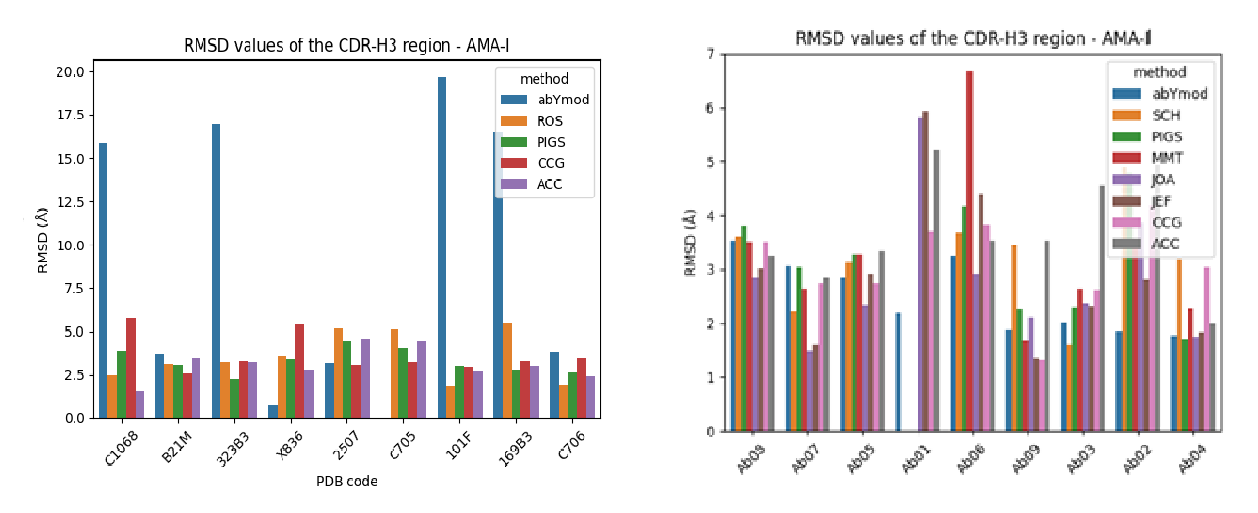
\includegraphics[width=\linewidth]{AMA.eps}
  \caption {RMSD values of the CDR-H3 loop for structures from the
    Antibody Modelling Assessment I (2011) and AMAII (2014). abYmod
    outperforms other modelling software in some instances, but also
    has much lower accuracy in few outlier cases. 
    Right: Ab01 is the rabbit antibody PDB:4MA3, which was
    excluded in the CDR-H3 modelling stage in AMAII due to
    difficulties modelling the overall structure previously. Ab01 is
    shown for the methods, where generated 3D-models were adequate for
    RMSD calculation.}
  \label{fig:AMA}
\end{figure}

The full pipeline for creating the final ML-model
starts with 
feature-set calculation using the antibody sequence. The feature set
includes attributes linked to sequence, structure, physical
characteristics, interactions, etc., within, as well as outside, the
loop. 
The sequence logo (Figure~\ref{fig:logo}) visualizes amino acid
occurrence within the loop sequence, elements of which can be
extracted as features \cite{Thomsen2012,Shaner1993}.

\begin{figure}
  \centering
  \includegraphics[width=\linewidth]{logo.eps}
  \caption {Sequence Logo of the CDR-H3 loop sequence. Data on amino
    acid occurrence taken from \protect\url{http://abymod.abysis.org/} Visualized
    using Seq2Logo using Kabat Numbering}
  \label{fig:logo}
\end{figure}

After creating the feature dataset, it is pre-processed (cleaning,
scaling, encoding, see methods for details). Structures with a
resolution worse than 4\AA\ were removed.
Instances of antibodies in our non-redundant dataset that matched in loop sequence were
not removed. 3D-Models of some of these structures with the same loop
sequence differ significantly. The few large RMSD ranges may stem from
low resolution. For example, the loop sequence with the largest RMSD range 
has multiple structure files linked to it of varying quality, one of which has a resolution of only 3.00\AA. Residue differences near the loop may also
explain the conformational difference of the loop itself, 
even if the loop sequence does not differ. Some of these structures are
complexed while others are not, which may also affect the loop
structure (manuscript in preparation).


The target data (i.e.\ RMSD values) are transformed from numerical
values to nominal values so that they can be used for
classification. In order to define these nominal categories, the total
RMSD range must be divided into categories. This is done either by
creating uniform classes i.e.\ 1--2\AA, 2--3\AA, etc., (the optimal size of which
must be determined), or by creating balanced classes. When
creating balanced classes, the upper and lower thresholds of a
category are chosen in such a way that each class contains an equal
number of instances. This approach was chosen to counteract the
skewness of the RMSD distribution. However, this was found to
affect the final ML-model's predictive power negatively. Therefore,
uniform classes were used.
The approach used is summarized in \ref{fig:nominal}

The RMSD values are also transformed into a set of binary values according to a
list of RMSD thresholds (i.e. a 1 is assigned to above and 0 to below a given threshold). This is done so that binary ML-models can be
trained, which will predict the probability e.g.\ that the 3D-model's RMSD
is above 2\AA, 2.2\AA, 2.4\AA, and so on. The number of binary
classifiers incorporated into the first layer has a great effect on
the final ML-model, the general trend being that the more binary
classifiers are used, the better the nominal prediction. 

\begin{figure}
  \centering
  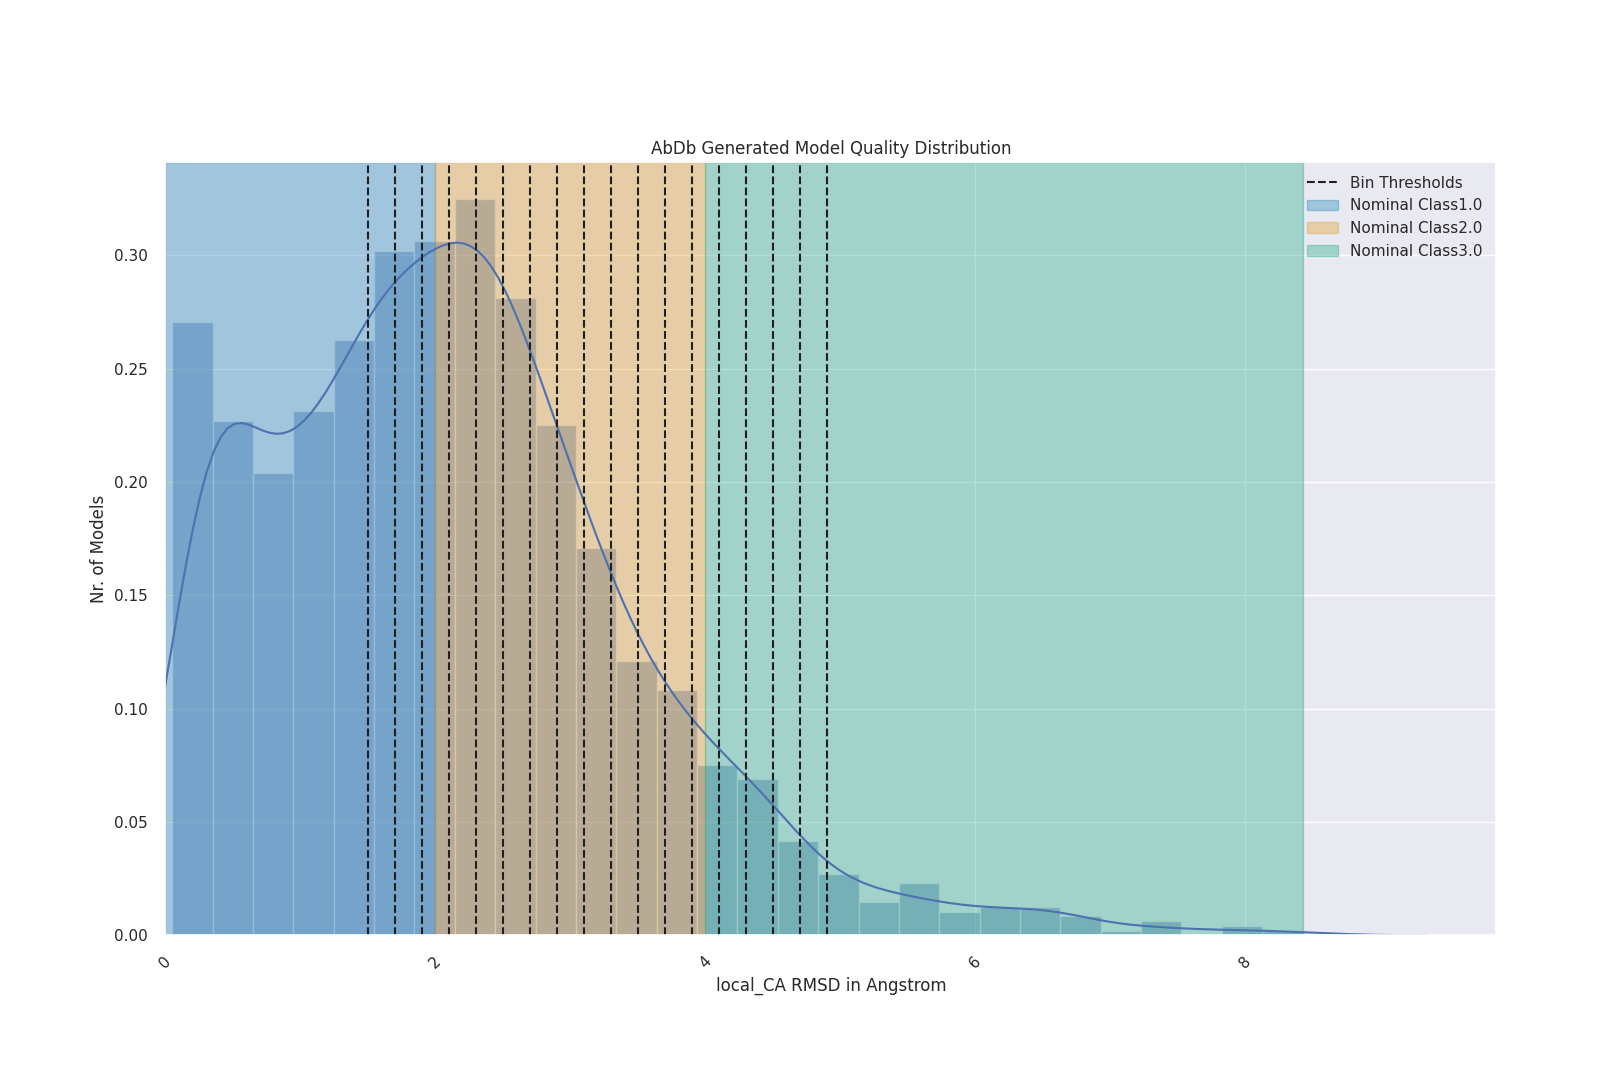
\includegraphics[width=\linewidth]{nominal_classes.png}
  \caption {Visualization of the binary and nominal categories used for the final predictor. The dotted lines mark the binary thresholds, while the coloured fields denote the nominal categories.}
  \label{fig:nominal}
\end{figure}


\subsection{Feature Encoding and Selection}

As some features are in the form of amino acid names, these must be
encoded before they can be passed to a ML-model. The
encoding strategy often determines how efficiently the ML-model learns
and how much information can be extracted. Different strategies were
employed to represent protein sequences numerically, such as BLOSUM62\cite{Henikoff1992} and NLF\cite{Nanni2011} encoding (a non-linear Fisher transform of a large set of physicochemical properties). The four-feature physiochemical encoding strategy\cite{Abhinandan2010} was implemented for all ML-models, being
the most effective. However, PCA-3 BLOSUM62, a dimensionality-reduced
BLOSUM62 encoding method achieved comparable results.
Feature selection was conducted to improve the ML-model's learning
capacity. A high-dimensional feature dataset bears the risk of
introducing excessive noise, facilitating ML-model over-fitting and can be
responsible for an overall decrease in ML-model performance and
stability. Each additional input feature forces the ML-model to
handle a more complex task, which consumes excess computational power
and time and provides more variables leading to over-fitting of the ML-model. 



Our ML-model was trained on different feature sets selected using manual
selection as well as algorithmic selection strategies (see methods), in order to
determine the most effective feature selection method. None of the
feature selection methods was a best fit for all ML-models. To create a ML-model implementing the encoding and feature selection strategies best suited for the specific ML-structure, a number of different combinations were tested, summarized in table \ref{results_table}. Additional ML-Models were discarded due to poor performance. 
\begin{table}[]
\fontsize{12}{16}\selectfont
  \centering
  \caption{Summary of Machine-Learning Classifier Performances}
  \label{results_table}

  \begin{adjustbox}{width=\textwidth}

    \begin{tabularx}{\linewidth}{
    |>{\hsize=.35\hsize}X|% 10% of 4\hsize 
    >{\hsize=.4\hsize}X|% 30% of 4\hsize
    >{\hsize=.4\hsize}X|% 30% of 4\hsize 
    >{\hsize=.4\hsize}X|% 30% of 4\hsize
    >{\hsize=.4\hsize}X|% 30% of 4\hsize 
    >{\hsize=.4\hsize}X|% 30% of 4\hsize
    >{\hsize=.2\hsize}X|% 30% of 4\hsize
       % sum=4.0\hsize for 4 columns
  }
\hline
Features & Feature Selection Method & Optimi-zation Method& Multi/ Single-layer & First-layer weighted &Classifier Type & MCC\\
\hline
Basic & None & None & single & No & SVC & 0.54\\
Basic & None & Genetic Algorithm & single & No & SVC & 0.54 \\
All & None & None & single& No & Random Forest & 0.58\\
Selected & random forest feature selection & Genetic Algorithm & Single& No & Soft Voting & 0.59 \\
Selected & random forest feature selection & Genetic Algorithm & Multi& Yes & XGB & 0.63 \\
Selected & recursive feature elimination & Genetic Algorithm & Multi& Yes & XGB & 0.79 \\
Selected & recursive feature elimination & Genetic Algorithm & Multi& Yes & XGB & 0.99 \\
Selected (no log-file features) & recursive feature elimination & Genetic Algorithm & Multi& Yes & Voting(soft) & 0.92 \\
\hline
    \end{tabularx}

  \end{adjustbox}

\end{table}
\caption{table caption}

The importance of the top features of the final models were ranked. This importance analysis clearly shows that loop length is the key feature for predicting the structural model quality \ref{fig:importance}. 
\begin{figure}
  \centering
  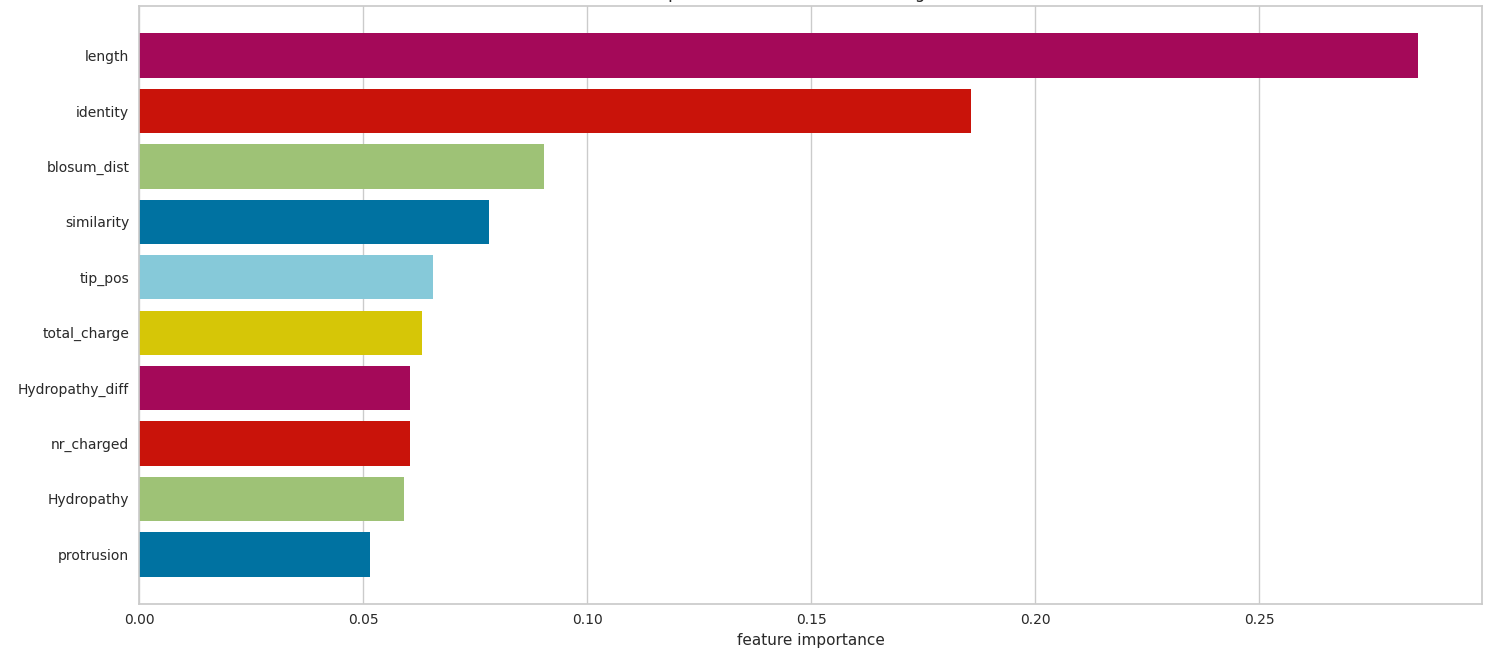
\includegraphics[width=\linewidth]{importance.png}
  \caption {Ranking of feature importance for the final model. The assigned values for importance were obtianed using the XGBoost package. \cite{Chen2016}}
  \label{fig:importance}
\end{figure}


After the data were processed, they were used to train different
ML-models. Different types of ML-model were investigated, as the most
suited ML-model type has to be determined heuristically. 
The following list, which includes some of the most commonly used
algorithms, was used: logistic regression, linear discriminant analysis,
K-nearest neighbours classifier, decision tree classifier, Gaussian
NB, random forest classifier, support vector machine,
probability-based voting (also known as soft voting) and extreme
gradient boosting (XGBoost)\cite{Chen2016}.

The best ML-model, and its best hyperparameters, are then determined for
each binary RMSD target. The set of binary ML-models outputs a number of
predictions that give the likelihood of the 3D-model having an RMSD above
the threshold value of the respective ML-model. These predictions are
then added to the feature set, on which a top-layer classifier is then
trained (Figure~\ref{fig:method}). Thus, a quasi-voting-system is incorporated into the final
classifier, in which a set of weaker classifiers vote on the ML-model
quality.

\subsection{Hyperparameter Optimization}
In the process of hyperparameter optimization, the configuration of
ML-model parameters which results in best performance is selected. This
is usually a computationally expensive and manual procedure.
In an effort to automate this process, a population was defined for
each ML-model type, so hyperparameter optimization could be conducted
automatically for each ML-model and seamlessly integrated into the full
ML-model creation process. Two different methods for hyperparameter
optimization were tested. The first was a hybrid approach of randomized
search and grid search; the second used a genetic algorithm for
optimization. The genetic algorithm was found to achieve slightly
better results and was employed for optimizing all ML-models.

\subsection{Machine Learning Model Performance}
The overall best final ML-model was composed of several different binary
classifiers, \ref{fig:flow} with an extreme gradient boosting (XGBoost) top-layer
nominal classifier. Features were selected using a recursive feature elimination algorithm, through which a the weakest feature is removed recursively and the model performance is tested. In the final model 9 features are included: in the final model, the following features were included: tip\_pos, protrusion, length, total\_charge, nr\_charged, identity, similarity, Hydropathy and Hydropathy\_diff \ref{fig:feature_table}.

A final MCC value of 0.99 could be achieved for an ML-model
using the abYmod log file as input as well as the loop 3D-model file
itself. This value slightly dropped to 0.92 if no such log file was
given. This is due to the fact that the template sequence
abYmod used to generate the 3D-model is unknown in the latter case.



The software
was tested on a test-set of antibody structures used in the 2014 and
2011 Antibody Modelling Assessments
\cite{Almagro2011,Almagro2014}. As the results depicted in
Figure~\ref{fig:AMA} show, abYmod achieves results similar to, or better than,
other modelling programs. However, the outliers with very high RMSD
values increase abYmod's RMSD average. The predictor in this work
would aim to identify such outlier 3D-models.


\begin{figure}
  \centering
  \includegraphics[width=\textwidth]{flowchart_qualiloop.eps}
  \caption {Simplified pipeline for creating the final machine learning model that will predict 3D-model quality by giving its RMSD range.}
  \label{fig:flow}
\end{figure}
 
\section{Methods}

\subsection{Computing}
All machine learning, feature selection and hyperparameter
optimization algorithms were implemented in Python. The Scikit-learn
library was used for training ML-models, the
Yellowbrick\cite{Bengfort2021} library was utilized for
visualization. All code is available at
\url{https://github.com/LilianDenzler/qualiloop}

The code was run under CentOS 7 on an 8-core virtual machine on an
Intel Xeon 4208 CPU with 16Gig RAM.

\subsection{Data Pre-Processing and Preparation}
Handling Null Values and Duplicates: The dataset containing target
RMSD values, and the calculated features was screened for null
values.
Rows that contained any null values were
removed from the dataset (11 rows in total).

\subsubsection{Duplicate Screening}
Using AbDb's redundancy information it was ensured that no antibodies
were present in the dataset more than once.

\subsubsection{Scaling}
Normalization and Standardization were tested as scaling methods. In normalization the range of the data is fixed between 0 and 1, while in Standardization the data is re-scaled to fit a Gaussian distribution. Both
approaches are greatly influenced by outliers, and such datapoints are
ideally removed for optimal scaling. Here we define outliers as
datapoints that lie over 1.5 times the interquartile range (IQR) below
the first quartile or above the third quartile. The IQR is defined as
the range between quartile 1, i.e.\ the median of the lower half of the
data, and quartile 3, i.e.\ the median of the upper half of the
data. However, across all features there are a total of 632 outlier
values and removing such a large number of datapoints is not a viable
option. A robust scaler\cite{XXXX} was also used, which uses statistics that are
robust to outliers. The median is set to zero and numerical features
are scaled to the interquartile range.

\subsubsection{BLOSUM 62 Encoding}
The BLOSUM62 matrix reflects the frequencies of amino acid
substitutions within a locally aligned, conserved regions of proteins
with at least 62\% similarity. Each amino acid is represented by a row
(or column) of the BLOSUM62 matrix. Dimensionality reduction
techniques were employed: Principal Component Analysis (PCA),
Independent Component Analysis (ICA), projection-based methods (t-SNE,
Isomap). Three components were used as features. PCA was found to be the most effective dimensionality reduction method. 

\subsubsection{Physiochemical Feature Encoding}
Martin and Abhinandan\shortcite{Abhinandan2010} introduced an encoding using
four physiochemical features:
the total number of sidechain atoms; the
number of sidechain atoms in the shortest path from the \ca\ to the most
distal atom; the Eisenberg consensus
hydrophobicity\cite{Eisenberg1982}; the charge (using +0.5 for histidine).

NLF-encoding \shortcite{Nanni2011} describes a new peptide encoding technique optimized for use with machine learning classifiers. A non-linear Fisher transform is applied to the whole set of physiochemical properties in \shortcite{Kawashima2000}
physiochemical properties are calculated and transformed using a
non-linear Fisher transform for dimensionality reduction.  A vector of
length 19 is produced for each amino acid.



\subsubsection{NLF Encoding}
This method of encoding is detailed by Nanni and Lumini in their paper. It takes many physicochemical properties and transforms them using a Fisher Transform (similar to a PCA) creating a smaller set of features that can describe the amino acid just as well. There are 19 transformed features. 

\subsection{Dataset-splitting}
The final ML-model was evaluated using a test set, separated from the
training set at the start in a 30/70 split. The performance of all individual sub-ML-models of the first layer was determined using stratified K-folds cross-validation (K=10) as the
dataset is imbalanced, being skewed towards lower RMSD values\cite{Krstajic2014,Kohavi1995}. The
method is different from normal K-folds cross validation as it uses
stratified sampling, which is also random, but selections are made to represent class imbalance.
This ensures each class is represented, as the percentage of samples for each class is
preserved.

\subsection{Machine Learning Model Assessment} 
ML-Model assessment must be considered at two levels as performance
metrics of binary and multi-class classifiers are calculated
differently and must thus be considered separately. The Matthews
Correlation Coefficient (MCC)\cite{Chicco2020} is deemed the most
informative, taking the ratios of the four confusion matrix categories
into account and is thus more reliable than the F1 score and
accuracy. It is also consistent for both binary and multi-class
problems and therefore well suited for our purpose.\cite{Jurman2012}
 
\subsection{Feature Calculations}

\begin{table}[]
  \centering
  \caption{A summary of how different feature values were calculated.}
  \label{fig:feature_table}

  \begin{adjustbox}{width=\textwidth}

    \begin{tabular}{| m{5em} | m{20em}| m{20em} |}
    \hline
Feature Name & Description & method of Calculation \\
\hline
\hline
Sequence & Amino acid sequence of the CDR-H3 loop. & Sequence is given in one-letter amino acid codes.\\
\hline
Length & Number of residues in the CDRH3-loop, which is located at residues H95-H102. & The number of residues are counted.\\
\hline
Sequence Identity & Sequence identity of selected template (SeqA) with input loop sequence (SeqB) is determined after sequence alignment. Calculated by abYmod during modelling. & $Identity(SeqA,SeqB) = 100\%\frac{identical residues}{length(alignment)}$\\
\hline
Sequence similarity & Sequence similarity of selected template (SeqA) with input loop sequence (SeqB) is determined after sequence alignment. Calculated by abYmod during modelling. Similar residues are residues that have undergone conservative substitution. &
$Similarity(SeqA,SeqB) = 100\%\frac{identical residues+similar residues}{length(alignment)}$\\
\hline
Loop Protrusion & Distance of loop residue further away from the loop base & Geometrical calculations \protect\ref{fig:loopdist} \\
\hline
Protruding residue & The Amino acid code of the most protruding loop residue & Using the previously determined point furthest away from the loop base, the residue at this coordinate is determined and given as a one-letter amino acid code.\\
\hline
Charge & Total charge of the loop & Sum of charges of all residues in loop \\
\hline
Charge difference & Difference in total charge compared to template sequence & Difference between the two summed changes \\
\hline
Hydrophobicity & Mean Hydrophobicity values of loop & Based on Eisenberg consensus values\\
\hline
Hydrophobicity  difference & Sum of absolute differences between loop sequence and template loop& Based on Eisenberg consensus values\\
\hline
Accessibility & Total and average accessibility for the loop& lee-Richards method implemented using the pdbsolv method from the BiopTools library.\\
\hline
Side-chain Accessibility & Total and average side-chain accessibility for the loop& lee-Richards method implemented using the pdbsolv method from the BiopTools library.\\
\hline
Relative Accessibility & Total and average relative accessibility for the loop& lee-Richards method implemented using the pdbsolv method from the BiopTools library.\\
\hline
relative side-chain Accessibility & Total and average relative side-chain accessibility for the loop& lee-Richards method implemented using the pdbsolv method from the BiopTools library.\\
\hline
Happiness & Happiness score, taking accessibility and hydropobicity into account. If a residue is 'happy' it will not be a buried hydrophilic or a surface hydrophobic residue. & Hydrophobicity values (see above) are normalized to a range of -1 to +1. Mean accessibility values are calculated as above. If hydrophobicity of loop is $<0$:
$Happiness = 1+Hydrophobicity(1-Accessibility)$
Otherwise:
$Happiness = 1-(Hydrophobicity Accessibility)$\\
\hline
Nr. of Contacts & Nr of contacts made by the residue of the loop within a range of 3.5\AA. Includes mainchain as well as sidechain atoms. Contacts made with residue within and outside of the loop are counted separately and as total. The ratio of inside vs outside is also calculated. & Modified version of the rangecontacts method in the BiopTools library. \\
\hline
Energy & Potential energy of the model. & Calculated by Gromacs during energy minimization step in abYmod modelling. \\
\hline
Lowest BLOSUM 62 Scoring Residue Pair & Each possible residue pair in the CDR-H3loop is scored by their BLOSUM 62 score. The lowest scoring pair's BLOSUM62 value will be combined with their residue separation to form the metric. & With separation being hte nuber of residues between the worst residue pair, and the worst score being the lowest BLOSUM62 score achieved by a residue pair, the metric is calculated as follows: $WorstBLOSUM = -log_2(separation)(worst score)$
\hline


    \end{tabular}

  \end{adjustbox}

\end{table}


\begin{figure}
  \centering
  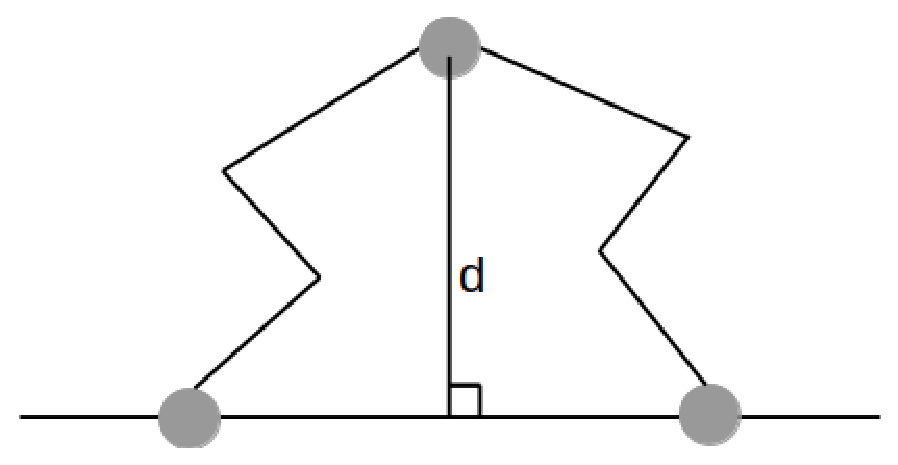
\includegraphics[scale=0.5]{protrusion.eps}
  \caption {Diagram
    visualizing the process underlying the protrusion
    calculation. First, the base residues (i.e.\ H95 and H102, shown as
    red spheres) of the CDR-H3 (grey circles) are identified. Then, a
    line is drawn between the two \ca\ atoms of these residues.
    The distance of the \ca-atom of each residue in the
    CDR-H3 loop to this line is calculated (d). The residue which has the
    greatest distance to the line is output
    as one-letter amino acid code and used as feature. The distance d in
    \AA\is used as the `protrusion'
    feature.}
  \label{fig:angle}
\end{figure}




\section{Discussion}
The results suggest that our classifier can differentiate
between well-modelled and less well-modelled CDR-H3 loop
structures. An MCC value of 0.99 was achieved, which underlines this
ability for accurate discrimination. Different methods for data
pre-processing, feature encoding, feature selection and hyperparameter
optimization were tested.
Feature encoding methods that were very high-dimensional
(one-hot-encoding, BLOSUM62, NLF) were found to be
unfavourable. Dimensionality reduction methods (Principal Component
Analysis (PCA), Independent Component Analysis (ICA), projection-based
methods e.g.\ t-SNE) were used on BLOSUM62 encoded matrices, which lead
to significant improvement. However, a physicochemical encoding
strategy was most effective.
The selection of features incorporated in the training set seemed to
be most important for effective learning. A multitude of methods were
tested. No one fit-for-all method for the different ML-models could be
found. However, for our top-layer classifier in our final ML-model
recursive feature elimination worked best.
A set of commonly used machine learning algorithms were tested, and
the best ML-models were incorporated into the final ensemble ML-model. A
stacked ML-model approach (consisting of 23 binary classifiers and a
single top-layer nominal classifier) was shown to outperform single
ML-models.
An MCC value of 0.99 was achieved for a classifier predicting whether
an input 3D-model has an RMSD value below 2\AA, 2\AA--4\AA\ or above
4\AA.

We are now looking at incorporating the predictor into the antibody
modelling process in the selection of high quality CDR-H3 models given
a set of potential decoys.

  
  
  

%\chapter{Future Directions}
\label{chapterlabel3}

\section{Make Stability Predictions}
1. Make stability predictions
-  Retrain antibody Tm-predictor on TCRs
-  Use melting-point library at immunocore
-  Sequence vs. structure based predictions
\section{Make Modifications}
2. Make modifications
-  Analyse packing residues
-  Compare to antibody packing residues
-  Reengineer to stabilize

\section{TCR Modelling}
extract features or structural rules to aid modelling
Alphafold testing
-  Domain Packing Prediction
-  Affinity enhancement
-  Tool for flagging unusual patches on surface
-  Deamidation prediction
Prevent degradation, enhance stability

\subsection{Martin-like Numbering}
Own numbering scheme, based on Kabat but with insertions and deletions at the structurally correct positions (Martin numbering)


%\addcontentsline{toc}{chapter}{Appendices}

% The \appendix command resets the chapter counter, and changes the chapter numbering scheme to capital letters.
%\chapter{Appendices}
\appendix
\chapter{An Appendix About Stuff}
\label{appendixlabel1}
(stuff)

\chapter{Another Appendix About Things}
\label{appendixlabel2}
(things)

\chapter{Colophon}
\label{appendixlabel3}
\textit{This is a description of the tools you used to make your thesis. It helps people make future documents, reminds you, and looks good.}

\textit{(example)} This document was set in the Times Roman typeface using \LaTeX\ and Bib\TeX , composed with a text editor. 
 % description of document, e.g. type faces, TeX used, TeXmaker, packages and things used for figures. Like a computational details section.
% e.g. http://tex.stackexchange.com/questions/63468/what-is-best-way-to-mention-that-a-document-has-been-typeset-with-tex#63503

% Side note:
%http://tex.stackexchange.com/questions/1319/showcase-of-beautiful-typography-done-in-tex-friends 
% You could separate these out into different files if you have
%  particularly large appendices.

% This line manually adds the Bibliography to the table of contents.
% The fact that \include is the last thing before this ensures that it
% is on a clear page, and adding it like this means that it doesn't
% get a chapter or appendix number.
\addcontentsline{toc}{chapter}{Bibliography}

% Actually generates your bibliography.
\bibliography{example}

% All done. \o/
\end{document}
